\documentclass{IEEEtran}
\usepackage{amsmath}
\usepackage{tikz}
\usepackage{pgfplots}
\usepackage[ruled,linesnumbered]{algorithm2e}

\begin{document}
\section{Environment}
\subsection{General parameters}
\begin{itemize}
    \item 100 by 100 meters squared area.
    \item 20 Users.
\end{itemize}
\subsection{User distribution}
\begin{itemize}
    \item The users are distributed around a local cluster.
    \item The center of the cluster is determined at random.
    \item It can take positions from 30 to 70, both in $x$ and $y$ coordinates.
    \item The users are scattered randomly with normal distribution around the cluster center, with mean $\mu = 0$ and standard deviation $\sigma = 20$.
    \item An example of the user distribution can be seen in Fig.~\ref{fig:users}.
\end{itemize}
\begin{figure}[h!]
    \resizebox{\columnwidth}{!}{% This file was created by matlab2tikz.
%
%The latest updates can be retrieved from
%  http://www.mathworks.com/matlabcentral/fileexchange/22022-matlab2tikz-matlab2tikz
%where you can also make suggestions and rate matlab2tikz.
%
\pgfplotsset{compat=1.3}
\def \mw {1.5pt}
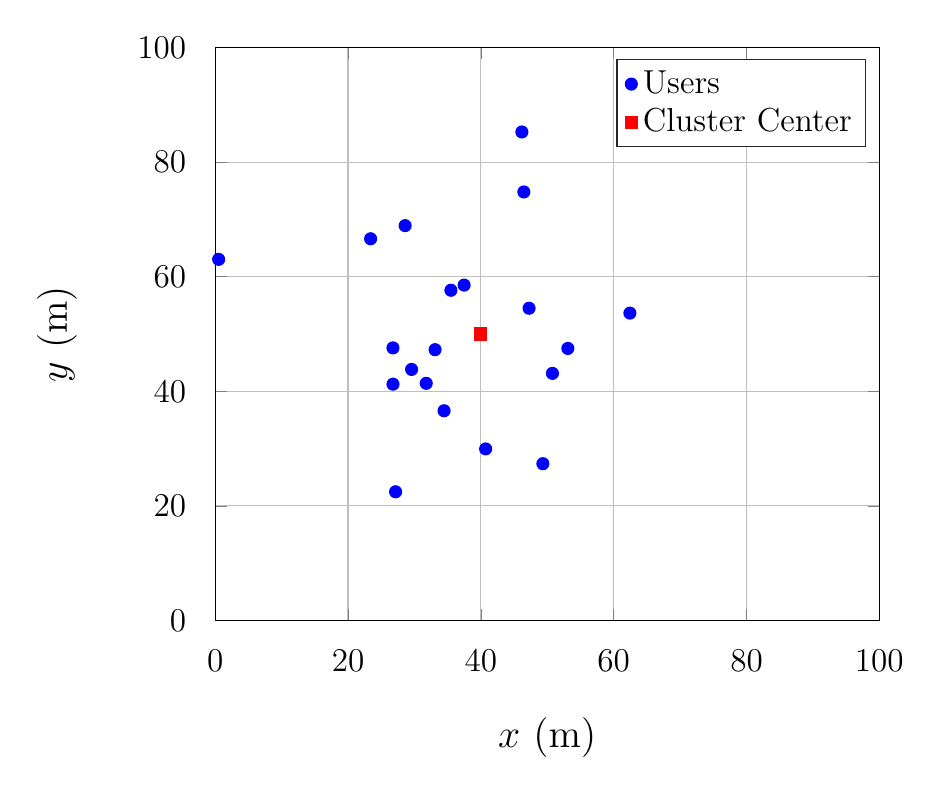
\begin{tikzpicture}

\begin{axis}[%
at={(0.13in,0.098in)},
scale only axis,
xmin=0,
xmax=100,
xlabel style={font=\color{white!15!black}},
xlabel={$x$ (m)},
ymin=0,
ymax=100,
ylabel style={font=\color{white!15!black}},
ylabel={$y$ (m)},
axis background/.style={fill=white},
xmajorgrids,
ymajorgrids,
minor grid style={dashed},
set layers,
xticklabel style = {font=\large, yshift=-.7em},
yticklabel style = {font=\large, xshift=-.7em},
xlabel style={font=\Large, yshift=-1em},
ylabel style={font=\Large, yshift=1.5em},
title style={font=\LARGE},
legend style={legend cell align=left, align=left, draw=white!15!black, font=\large},
]
\addplot[only marks, mark=*, mark options={}, mark size=2.1651pt, draw=blue, fill=blue] table[row sep=crcr]{%
x	y\\
33.1039363358315	47.2670913994937\\
40.7188405447753	29.9435329451968\\
62.4424298818045	53.6514820435643\\
46.4736717181615	74.7995213752686\\
31.7755815671182	41.3952752335151\\
27.1642791732632	22.4610412525807\\
26.7703062136752	41.2448653155578\\
35.4948422927757	57.6370351284124\\
23.4023317642292	66.6269214324328\\
37.4768531424445	58.5426309921738\\
46.1748050049962	85.2705873537184\\
28.5983093592481	68.9146276316762\\
50.7767022293099	43.1297066818567\\
49.3371914257899	27.3643931702637\\
0.518481083217345	63.0339329356793\\
47.2591243548809	54.5002811092411\\
26.7652048499168	47.5772814799484\\
34.4591526968066	36.6033425669962\\
29.5731235540687	43.8203152787121\\
53.0980857004862	47.483272921902\\
};
\addlegendentry{Users};

\addplot[only marks, mark=square*, mark size=2.1651pt, draw=red, fill=red] table[row sep=crcr]{%
x y \\
40 50 \\
};
\addlegendentry{Cluster Center};


\end{axis}
\end{tikzpicture}%
}
    \caption{Example of user distribution in one training session.}\label{fig:users}
\end{figure}
\subsection{Drones}
\begin{itemize}
    \item The drones are assumed to have ideal communication among themselves.
    \item The drones share their positions and number of users allocated with each other.
    \item Each drone has a directional antenna with a main lobe with an aperture angle of $\theta=60$ degrees. The antenna is pointing downwards. An illustration of the directivity angle is presented in Fig.~\ref{fig:angle}
        \begin{figure}
            \centering
            \resizebox{.5\columnwidth}{!}{\begin{tikzpicture}[scale=1]
    %Include eps images
    \node (im2) at (0,5) {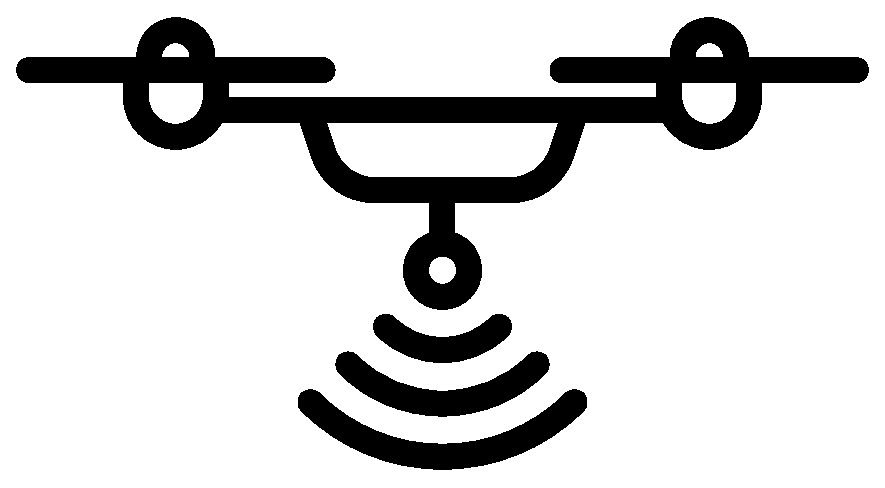
\includegraphics[trim={0 77 0 0},clip,scale = 0.5,width=10em]{drone.eps}};

    \coordinate (A) at (im2.south);
    \coordinate (X) at (0,-3);
    \coordinate (Y) at (4,-3);
    
    \draw[line width=0.75mm,dashed] (X) -- (A) -- (Y);

    \draw [line width=0.75mm] (im2.south) -- (X);
    \node (t1) at (0.5,0) {\LARGE $h_\text{d}$};

    \begin{scope}
        \path[clip] (A) -- (X) -- (Y);
        \fill[gray, opacity=0.5, draw=black, thick] (A) circle (5em);
    \end{scope}
    %\node at ($(A)+(1em,-2em)$) {$\theta/2$};
    \node (ang) at (0.5,2) {\huge $\frac{\theta}{2}$};
    \draw [line width=0.75mm, dashed](0,-3) ellipse (4 and 1);
    \node (t2) at (0,-4.5) {\LARGE Footprint};
\end{tikzpicture}
}
            \caption{Illustration of the coverage radius of a drone flying at $h_\text{d}$ meters and with directivity angle of $\theta$.}\label{fig:angle}
        \end{figure}
    \item There is no limit on the number of users that each drone can allocate.
    \item Each drone is assumed to be flying at a fixed height ${h_\text{d} = 30}$ meters.
\end{itemize}
\section{States}
\begin{itemize}
    \item The states are the positions of both drones.
    \item The environment is discretized into 121 possible positions for each drone (steps of 10 meters).
    \item Drones cannot assume the same position at the same time.
    \item The total number of states is therefore $2 \times \binom{121}{2} = 14520$.
\end{itemize}
\section{Actions}
\begin{itemize}
    \item The possible actions are to move $\pm 1$ step in $x$ or $y$.
    \item If one drone would move to the same position as the other (e.g\. chooses the action to move right when the other drone is one step to its right), it does not move.
    \item If a drone would move out of the grid (e.g\. chooses to move right when at $x$ coordinate 100), it does not move.
    \item If a state has not been explored, the action is also chosen at random, in order to avoid bias.
    \item Otherwise, actions are deterministic.
\end{itemize}
\section{Policy}
\begin{itemize}
    \item The policy is $\varepsilon$-greedy.
    \item Meaning that each drone chooses a random action with probability $\varepsilon$ and $\max (Q_{s_{t+1}, *})$ with probability $1 - \varepsilon$.
\end{itemize}
\section{Reward}
\begin{itemize}
    \item The reward is the total number of users allocated by both drones.
\end{itemize}
\subsection{User Association}
\begin{itemize}
    \item A user associates with a drone if its received SINR is above a threshold of 40 dB.
    \item The SINR for the link between user $u$ and drone $n$ is calculated according to
        \begin{equation}
            SINR_{n,u} = \frac{RSRP_{n, u}}{N + \sum_{\forall i \neq n} RSRP_{i, u}}.
        \end{equation}
    \item The RSRP for the link between user $u$ and drone $n$ is calculated according to the free space path loss, as
        \begin{equation}
            RSRP_{n,u} = \frac{P_\text{t}}{\frac{16 {(\pi  f_\text{c} d)}^2}{c^2}},
        \end{equation}
        where $c$ is the speed of light in meters per second, $P_\text{t}$ is the drone transmit power in Watts and $f_\text{c}$ is the carrier frequency in Hz.
    \item Any user outside the main lobe is considered to receive 0 W of power from the drone.
\end{itemize}
\section{Training}
\begin{itemize}
    \item The training session is comprised of 100 episodes of 20,000 iterations each.
    \item The state of the drones is set randomly at the beginning of each episode.
    \item $\varepsilon$ decays exponentially with the episode number, according to:
        \begin{equation}
            \varepsilon_j = \mathrm{e}^{-j/20},
        \end{equation}
        where $j$ is the episode number and $\mathrm{e}$ is Euler's constant.
\end{itemize}
\subsection{Algorithm}
The update strategy for SARSA is expressed as
\begin{equation}
    \begin{align}
        Q(s_t, a_t, \delta) = Q(s_t, a_t, \delta) &+ \\ \alpha (r_t + \gamma Q(s_{t+1},& a_{t+1}, \delta) - Q(s_t, a_t, \delta)),
    \end{align}
\end{equation}
where $\alpha$ is the learning rate and $\gamma$ is the discount factor.
A pseudo code of the implemented solution is presented in Algorithm~\ref{alg:SARSA}.
\begin{algorithm}[h]
    \SetKwFunction{random}{random}
    \SetKwFunction{chooseAction}{chooseAction}
    \SetKwFunction{takeAction}{takeAction}
    \SetKwFunction{computeReward}{computeReward}
    \SetKwFunction{updateQ}{updateQ}
        Initializations \\
    \For{Every episode $j$} {%
        $s_1$ \leftarrow~\random(1, 14520) \\
        \For{Every iteration $t$} {%
            \For{Every drone $\delta$} {%
                $a_t$ \leftarrow~\chooseAction($Q_{s_t,*}$, $\varepsilon_j$, $\delta$) \\
                $s_{t+1}$ \leftarrow~\takeAction($s_t$, $a_t$, $\delta$) \\
                $a_{t+1}$ \leftarrow~\chooseAction($Q_{s_{t+1},*}$, $\varepsilon_j$, $\delta$) \\
                $r_t$ \leftarrow~\computeReward($s_{t+1}$) \\
                $Q(s_t, a_t, d)$ \leftarrow~\updateQ()\\
                $s_t$ \leftarrow~$s_{t+1}$ \\
            }
        }
    }
\caption{SARSA implementation}\label{alg:SARSA}
\end{algorithm}
\section{Results}
The average reward per episode is shown in Fig.~\ref{fig:results}.
\begin{figure}[t!]
    \resizebox{\columnwidth}{!}{% This file was created by matlab2tikz.
%
%The latest updates can be retrieved from
%  http://www.mathworks.com/matlabcentral/fileexchange/22022-matlab2tikz-matlab2tikz
%where you can also make suggestions and rate matlab2tikz.
%
\pgfplotsset{compat=1.3}
\definecolor{mycolor1}{rgb}{0.00000,0.44700,0.74100}%
\definecolor{mycolor2}{rgb}{0.85000,0.32500,0.09800}%
\definecolor{mycolor3}{rgb}{0.92900,0.69400,0.12500}%
%
\begin{tikzpicture}

\begin{axis}[%
width=4.521in,
height=3.566in,
at={(0.758in,0.481in)},
scale only axis,
xmin=0,
xmax=100,
xlabel style={font=\color{white!15!black}},
xlabel={Episode $j$},
ymax=18,
ylabel style={font=\color{white!15!black}},
ylabel={Average Reward $r$},
axis background/.style={fill=white},
xmajorgrids,
ymajorgrids,
legend style={legend cell align=left, align=left, draw=white!15!black},
legend style={at={(.8,.2)}, anchor = center},
minor grid style={dashed},
set layers,
xticklabel style = {font=\large, yshift=-.7em},
yticklabel style = {font=\large, xshift=-.7em},
xlabel style={font=\Large, yshift=-1em},
ylabel style={font=\Large, yshift=1.5em},
legend style={font=\large},
title style={font=\LARGE},
mark repeat=5,
]
\addplot [color=mycolor1, line width=2.0pt, mark size=5pt, mark options={solid, line width=\mw, fill=white}]
  table[row sep=crcr]{%
1	4.157075\\
2	3.579275\\
3	4.18365\\
4	4.63545\\
5	5.35475\\
6	6.05725\\
7	6.7247\\
8	7.641525\\
9	8.372325\\
10	8.9307\\
11	9.3931\\
12	9.98945\\
13	10.288075\\
14	10.94685\\
15	11.437975\\
16	11.73375\\
17	12.18995\\
18	12.35205\\
19	12.62035\\
20	12.891225\\
21	13.024275\\
22	13.2074\\
23	13.3787\\
24	13.493325\\
25	13.59985\\
26	13.689575\\
27	13.937425\\
28	14.021375\\
29	14.09635\\
30	14.1076\\
31	14.140675\\
32	14.363025\\
33	14.261575\\
34	14.357025\\
35	14.4147\\
36	14.522875\\
37	14.6616\\
38	14.659275\\
39	14.697825\\
40	14.733825\\
41	14.77385\\
42	14.8961\\
43	14.970325\\
44	15.0237\\
45	14.981925\\
46	15.0275\\
47	15.11975\\
48	15.116175\\
49	15.14305\\
50	15.004\\
51	15.224025\\
52	15.303425\\
53	15.08265\\
54	15.081225\\
55	15.1922\\
56	15.171075\\
57	15.237875\\
58	15.27115\\
59	15.5189\\
60	15.118225\\
61	15.153775\\
62	15.2042\\
63	15.275725\\
64	15.2645\\
65	15.379575\\
66	15.349975\\
67	15.3702\\
68	15.45665\\
69	15.46775\\
70	15.666575\\
71	15.563425\\
72	15.63275\\
73	15.7093\\
74	15.37795\\
75	15.3026\\
76	15.6765\\
77	15.403375\\
78	15.50205\\
79	15.286075\\
80	15.3936\\
81	15.528\\
82	15.54455\\
83	15.6641\\
84	15.53775\\
85	15.632375\\
86	15.520175\\
87	15.3686\\
88	15.50565\\
89	15.52705\\
90	15.611375\\
91	15.569675\\
92	15.452025\\
93	15.35395\\
94	15.55555\\
95	15.77065\\
96	15.628875\\
97	15.6255\\
98	15.848975\\
99	15.739325\\
100	15.2568\\
};
\addlegendentry{Avg reward}

\addplot [color=mycolor3, line width=2.0pt, dotted]
  table[row sep=crcr]{%
1	16\\
2	16\\
3	16\\
4	16\\
5	16\\
6	16\\
7	16\\
8	16\\
9	16\\
10	16\\
11	16\\
12	16\\
13	16\\
14	16\\
15	16\\
16	16\\
17	16\\
18	16\\
19	16\\
20	16\\
21	16\\
22	16\\
23	16\\
24	16\\
25	16\\
26	16\\
27	16\\
28	16\\
29	16\\
30	16\\
31	16\\
32	16\\
33	16\\
34	16\\
35	16\\
36	16\\
37	16\\
38	16\\
39	16\\
40	16\\
41	16\\
42	16\\
43	16\\
44	16\\
45	16\\
46	16\\
47	16\\
48	16\\
49	16\\
50	16\\
51	16\\
52	16\\
53	16\\
54	16\\
55	16\\
56	16\\
57	16\\
58	16\\
59	16\\
60	16\\
61	16\\
62	16\\
63	16\\
64	16\\
65	16\\
66	16\\
67	16\\
68	16\\
69	16\\
70	16\\
71	16\\
72	16\\
73	16\\
74	16\\
75	16\\
76	16\\
77	16\\
78	16\\
79	16\\
80	16\\
81	16\\
82	16\\
83	16\\
84	16\\
85	16\\
86	16\\
87	16\\
88	16\\
89	16\\
90	16\\
91	16\\
92	16\\
93	16\\
94	16\\
95	16\\
96	16\\
97	16\\
98	16\\
99	16\\
100	16\\
};
\addlegendentry{Exhaustive Search}

\end{axis}
\end{tikzpicture}%
}
    \caption{Average reward per episode considering for this training session}\label{fig:results}
\end{figure}
\end{document}


